\documentclass[10pt, letterpaper]{article}
%Graphic and Diagram Setup
\usepackage[margin=1in]{geometry}
\usepackage{graphicx}
\usepackage{tikz}
\usepackage[all]{xy}

\usepackage{pdflscape}
\usepackage{rotating}

%Inserting Graphics
%An example of the use of this command is
% \begin{minipage}{4in}
%   \Fig{filename}
% \end{minipage}
\newcommand{\Fig}[1]{\includegraphics[width=0.5\textwidth]{#1}}

%Math Symbol Setup
\usepackage{ulem}
\usepackage{amsmath}
\usepackage{amsthm}
\usepackage{amssymb}

%Math Fonts
\usepackage{amsfonts}
\usepackage{mathrsfs}

%Absolute Value and Norm Notation
\newcommand{\abs}[1]{\left \lvert #1 \right \rvert}
\newcommand{\norm}[1]{\left \lVert #1 \right \rVert}

%Kernel of a map
\renewcommand{\ker}{\operatorname{Ker}}

%Lie Algebra of a Lie Group
\newcommand{\lie}[1]{\operatorname{Lie}(#1)}

%Fields and Blackboard Letters
\newcommand{\field}[1]{\mathbb{#1}}
\newcommand{\A}{\mathbb{A}}
\renewcommand{\P}{\mathbb{P}}
\newcommand{\N}{\mathbb{N}}
\newcommand{\Z}{\mathbb{Z}}

%Theorems and Definitions
\newtheorem{thm}{Theorem}
\newtheorem{lemma}{Lemma}
\newtheorem{cor}{Corollary}
\newtheorem{prop}{Proposition}

\theoremstyle{remark}
\newtheorem{rem}{Remark}

\theoremstyle{definition}
\newtheorem{defn}{Definition}
\newtheorem{ex}{Example}

%Fancy Header Setup
\usepackage{fancyhdr}
\fancyhf{}
\pagestyle{fancy}
\lhead{}
\chead{\bfseries Graph Theory}
\rhead{}
\lfoot{Linear Algebra \& Graph Theory}
\cfoot{Eric Ebert}
\rfoot{\thepage}
\renewcommand{\headrulewidth}{0.5pt}
\renewcommand{\footrulewidth}{0.1pt}

%Double Space
\usepackage{setspace}
\linespread{1.6}

%Document Content
\begin{document}

\section{Set Theory}

We begin with some reminders from set theory. We make no attempt to be exacting and take the intuitive approach as demonstrated in Robert Stoll's book. We let $A$ and $B$ be two arbitrary sets.

\begin{defn}
	The relative complement of $B$ from $A$ is the set
	\[
		A - B = \{a \in A \mid a \notin b\}
	\]
\end{defn}

Notice that if the two sets are disjoint ($A \cap B = \emptyset$) then $A-B=A$. We now use this concept to define the \textit{symmetric difference}.

\begin{defn}
	The symmetric difference $A + B$ is defined to be the set
	\[
		A + B = (A - B) \cup (B - A)
	\]
\end{defn}

After pondering this a bit, one realizes that $A+B$ is simply the set of objects that belong to one of the sets but not both.

\begin{rem} \leavevmode
	\begin{itemize}
		\item Some books use the notation $A \bigtriangleup B$ for the symmetric difference.
		\item If you're hoping that the notation $A+B$ is going to lead to an abelian group, you're in luck. 
		\item $A+B = (A \cup B) - (A \cap B)$.
	\end{itemize}
\end{rem}

We now recall the \textit{power set} $\mathcal{P}(A)$ of a set $A$. The power set consists of all subsets of $A$. This is in bijection with all functions $A \rightarrow \field{F}_2$, where $\field{F}_2 \cong \Z/2\Z$ the field of two elements. This is often denoted by $\field{F}_2^A$ or $\{0,1\}^A$. Each subset of $A$ say $S=\{a_1, a_2, \ldots, a_k\}$ is identified with the function $1_S: A \rightarrow \field{F}_2$ which assigns $1$ to each $a_i \in S$ and zero to all other elements of $A$. This is referred to as the \textit{indicator function} of $S$.

\begin{prop}
	Let $A$, $B$ and $C$ be three arbitrary sets that live in a universe $U$. Then
	\begin{enumerate}
		\item[(a)] \textbf{Closure: }$A+B$ is a subset of $U$.
		\item[(b)] \textbf{Associative: } $(A+B)+C = A+(B+C)$.
		\item[(c)] \textbf{Identity: } $A + \emptyset = A = \emptyset + A$.
		\item[(d)] \textbf{Inverse: } $A + A = \emptyset$.
	\end{enumerate}
\end{prop}

\begin{rem} \leavevmode
	\begin{itemize}
		\item Using the proposition one gets what was eluded to above; that the power set is an abelian group under the operation of the symmetric difference.
		\item One can extend this to obtain a \textit{boolean ring} by using $\cap$ as the multiplication.
		\item The property in (d) yields that every element is nilpotent.
	\end{itemize}
\end{rem}

Now let $S \in \mathcal{P}(A)$. One can define an action of $\field{F}_2$ on $\mathcal{P}(A)$ by $0 \cdot S = \emptyset$ and $1 \cdot S = S$. It is a standard exercise to show that this action is compatible with the operation of symmetric difference. 

\hspace*{.15in}

\textbf{Conclusion: } The power set can be viewed as a vector space over $\field{F}_2$.

\section{Vector Spaces \& Graphs}

Let $G = (V,E)$ be a graph where $V$ is the set of vertices and $E$ is the set of edges. We are considering undirected graphs where the cardinality of $V$ and $E$ are finite. One defines $\mathcal{V}(V) = \{0,1\}^V$ and $\mathcal{V}(E) = \{0,1\}^E$ to be the \textit{vertex space} and \textit{edge space}. Given that any subset of $V$ can be written as the sum (symmetric difference) of the individual unit subsets
\[
	\{v_{i_1}, v_{i_2}, \ldots, v_{i_k}\} = \{v_{i_1}\} + \{v_{i_2}\} + \cdots + \{v_{i_k}\}
\]
we conclude that the set of $\{\{v_i\} \mid v_i \in V\}$ is a basis for the vertex space and that it is finite-dimensional with dimension \#$V$. Everything done here for the vertex space can be done analagously for the edge space.

\section{Matrices}

We will be using the following graph in our discussion:

\vspace*{.15in}

\begin{figure}
\centering
	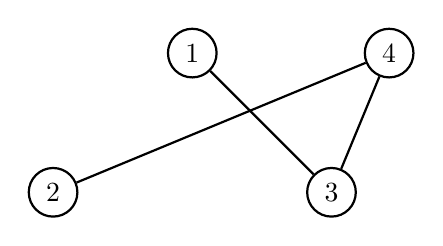
\begin{tikzpicture}[node distance={25mm}, thick, main/.style={draw,circle}]
		\node[main] (1) {$1$};
		\node[main] (2) [below left of = 1] {$2$};
		\node[main] (3) [below right of = 1] {$3$};
		\node[main] (4) [right of = 1] {$4$};
		
		\draw (1) -- (3);
		\draw (2) -- (4);
		\draw (3) -- (4);
	\end{tikzpicture}
	\caption{Graph with no cycle}
\end{figure}

Notice that the vertex space is four dimensional and has standard basis $v_1=\{1\}, v_2=\{2\}, v_3=\{3\}, v_4=\{4\}$ and the edge space is three dimensional and has standard basis $e_1=\{(1,3)\}, e_2=\{(2,4)\}, e_3=\{(3,4)\}$.


\subsection{The incidence matrix $B$}
We now define the \textit{incidence matrix} $B=(b_{ij})$ to be
\[
	b_{ij} = \begin{cases}
				1 &\text{ if } v_i \in e_j \\
				0 &\text{ otherwise}
			 \end{cases}
\]

Notice that this will yield a linear map $B: \mathcal{V}(E) \rightarrow \mathcal{V}(V)$. For our graph we have the following incidence matrix:
\[
	B = \begin{pmatrix}
		1 & 0 & 0 \\
		0 & 1 & 0 \\
		1 & 0 & 1 \\
		0 & 1 & 1 \\
	\end{pmatrix}
\]

\begin{ex}
The vector $(0,1,0)^T$ corresponds to $e_2$ and 
\[
	Be_1 = \begin{pmatrix}
		1 & 0 & 0 \\
		0 & 1 & 0 \\
		1 & 0 & 1 \\
		0 & 1 & 1 \\
	\end{pmatrix}
	\begin{pmatrix}
		0 \\ 1 \\ 0 \\
	\end{pmatrix} =
	\begin{pmatrix}
		0 \\ 1 \\ 0 \\ 1 \\
	\end{pmatrix}
\]
The image vector corresponds to the 2nd and 4th vertices, which are the vertices incident to $e_2$. We now understand the action of $B$ on any basis element of the edge space: we get the vertices that for then end points of the edge.
\end{ex}

\begin{ex}
Now notice that $e_1 \text{ and } e_2$ are a \textit{matching} of the given graph. That is the edges $e_1$ and $e_2$ are independent in the sense that the edges account for every vertex and no two edges are adjacent to each other.

\[
	\begin{pmatrix}
		1 & 0 & 0 \\
		0 & 1 & 0 \\
		1 & 0 & 1 \\
		0 & 1 & 1 \\
	\end{pmatrix}
	\begin{pmatrix}
		1 \\ 1 \\ 0 \\
	\end{pmatrix} =
	\begin{pmatrix}
		1 \\ 1 \\ 1 \\ 1 \\
	\end{pmatrix}
\]

The image of $B$ in this case yields every vertex.
\end{ex}

\begin{ex}
	Now we consider the path from $v_1=\{1\} \text{ to } v_4=\{4\}$ via $e_1$ and $e_3$. Then
	\[
		\begin{pmatrix}
		1 & 0 & 0 \\
		0 & 1 & 0 \\
		1 & 0 & 1 \\
		0 & 1 & 1 \\
	\end{pmatrix}
	\begin{pmatrix}
		1 \\ 0 \\ 1 \\
	\end{pmatrix} =
	\begin{pmatrix}
		1 \\ 0 \\ 0 \\ 1 \\
	\end{pmatrix}
	\]
	
Remember we are doing the multiplication mod 2. We are unsurprised that vertex $\{2\}$ is left our because it is not in our path. Notice that the other vertex that was left out ($\{3\}$) has even degree (in our path) as we entered and left this vertex.
\end{ex}

\begin{rem}
	In our example, $B$ has full rank and therefore the map associated to $B$ has trivial kernel. 
\end{rem}

Let's modify our graph by adding an edge $e_4 = (1,4)$.

\begin{figure}
\centering
	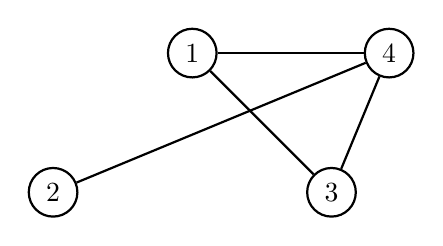
\begin{tikzpicture}[node distance={25mm}, thick, main/.style={draw,circle}]
		\node[main] (1) {$1$};
		\node[main] (2) [below left of = 1] {$2$};
		\node[main] (3) [below right of = 1] {$3$};
		\node[main] (4) [right of = 1] {$4$};
		
		\draw (1) -- (3);
		\draw (1) -- (4);
		\draw (2) -- (4);
		\draw (3) -- (4);
	\end{tikzpicture}
	\caption{Graph with a cycle; edge $e_4$ added}
\end{figure}

We now have the following incidence matrix:
\[
	B = \begin{pmatrix}
		1 & 0 & 0 & 1 \\
		0 & 1 & 0 & 0 \\
		1 & 0 & 1 & 0 \\
		0 & 1 & 1 & 1 \\
	\end{pmatrix}
\]

\begin{ex}
	We are going to consider the cycle beginning and ending at $v_1=\{1\}$ via the simple path $e_1, e_3, \text{ and } e_4$.
	\[
		\begin{pmatrix}
		1 & 0 & 0 & 1 \\
		0 & 1 & 0 & 0 \\
		1 & 0 & 1 & 0 \\
		0 & 1 & 1 & 1 \\
	\end{pmatrix}
	\begin{pmatrix}
		1 \\ 0 \\ 1 \\ 1
	\end{pmatrix} = 
	\begin{pmatrix}
		0 \\ 0 \\ 0 \\ 0
	\end{pmatrix}
	\]
	In this example, the incidence matrix has sent our cycle to zero. We note that every node in our cycle has even degree.
\end{ex}

\begin{ex}
 Here we take a path from vertex $\{2\}$ to vertex $\{4\}$ using all of the edges:
 \[
 	\begin{pmatrix}
		1 & 0 & 0 & 1 \\
		0 & 1 & 0 & 0 \\
		1 & 0 & 1 & 0 \\
		0 & 1 & 1 & 1 \\
	\end{pmatrix}
	\begin{pmatrix}
		1 \\ 1 \\ 1 \\ 1
	\end{pmatrix} = 
	\begin{pmatrix}
		0 \\ 1 \\ 0 \\ 1
	\end{pmatrix}
 \]
 The image here yields vertex 2 and vertex 4. The two vertices in the graph with odd degree.
\end{ex}

\begin{prop}
	The linear map $B: \mathcal{V}(E) \rightarrow \mathcal{V}(V)$ takes an edge set to the set of vertices incident to an odd number of edges in the preimage. In other words, if $F \subset E$ then the image of $B$ on $F$ picks out the vertices which are incident to an odd number of vertices in $F$.
\end{prop}

\subsection{The dual $B^T$}
Given a matrix and its associated taking the transpose gives us the dual map. We ask: what role does it play? We begin by noting that $B^T$ will define a linear map $\mathcal{V}(V) \rightarrow \mathcal{V}(E)$.

\begin{ex}
	Let's consider the vertex $\{1\}$ and compute $B^Tv_1$:
	\[
		\begin{pmatrix}
			1 & 0 & 1 & 0 \\
			0 & 1 & 0 & 1 \\
			0 & 0 & 1 & 1 \\
		\end{pmatrix}
		\begin{pmatrix}
			1 & 0 & 0 & 0 \\
		\end{pmatrix} = 
		\begin{pmatrix}
			1 \\ 0 \\ 0 
		\end{pmatrix}
	\]
	The edge we've labeled $e_1$ is the only edge with $v_1=\{1\}$ as an endpoint.
\end{ex}

\begin{ex}
	Now let's look at $v_4 = \{4\}$.
	\[
		\begin{pmatrix}
			1 & 0 & 1 & 0 \\
			0 & 1 & 0 & 1 \\
			0 & 0 & 1 & 1 \\
		\end{pmatrix}
		\begin{pmatrix}
			0 & 0 & 0 & 1 \\
		\end{pmatrix} = 
		\begin{pmatrix}
			0 \\ 1 \\ 1 
		\end{pmatrix}
	\]
	Here the image has selected the two edges we've labeled $e_2 \text{ and } e_3$. These are the two edges incident to $v_4$.
\end{ex}

\begin{ex}
	Let's now consider $U = \{v_3,v_4\}$ and find the image of $U$ under $B^T$
	\[
		\begin{pmatrix}
			1 & 0 & 1 & 0 \\
			0 & 1 & 0 & 1 \\
			0 & 0 & 1 & 1 \\
		\end{pmatrix}
		\begin{pmatrix}
			0 & 0 & 1 & 1 \\
		\end{pmatrix} = 
		\begin{pmatrix}
			1 \\ 1 \\ 0 
		\end{pmatrix}
	\]
	The edges $e_1$ and $e_2$ are the edges in the image. Notice that $e_3$ has been left out as both of the vertices in $U$ form that edge.
\end{ex}

\begin{prop}
	The matrix $B^T$ defines a map $\mathcal{V}(V) \rightarrow \mathcal{V}(E)$ which maps a subset of vertices $U \subset V$ to the edges with exactly one vertex in $U$.
\end{prop}

\subsection{The Quadratic form $BB^T$}
We return to our original incidence matrix.  We now compute $BB^T$:
\[
	BB^T = \begin{pmatrix}
		1 & 0 & 0 \\
		0 & 1 & 0 \\
		1 & 0 & 1 \\
		0 & 1 & 1 \\
	\end{pmatrix}
	\begin{pmatrix}
		1 & 0 & 1 & 0 \\
		0 & 1 & 0 & 1 \\
		0 & 0 & 1 & 1 \\
	\end{pmatrix} =
	\begin{pmatrix}
		1 & 0 & 1 & 0 \\
		0 & 1 & 0 & 1 \\
		1 & 0 & 2 & 1 \\
		0 & 1 & 1 & 1 \\
	\end{pmatrix} =
	\begin{pmatrix}
		0 & 0 & 1 & 0 \\
		0 & 0 & 0 & 1 \\
		1 & 0 & 0 & 1 \\
		0 & 1 & 1 & 0 \\
	\end{pmatrix} +
	\begin{pmatrix}
		1 \\
		 & 1 \\
		 & & 2 \\
		 & & & 2 \\
	\end{pmatrix}
\]

We can reduce the entries to mod 2 as we have been doing. However, we want to make a couple of observations here:

\begin{enumerate}
	\item[(a)] The diagonal matrix has entries $d_{ii}$ the degree of $v_i$, $i=1,2,3,4$.
	\item[(b)] The left summand is the adjacency matrix as defined below.
	\item[(c)] $BB^T$ is a symmetric matrix and diagonally dominant and is therefore positive semidefinite..
\end{enumerate}

\subsection{Adjacency Matrix}

We now formally define the adjacency matrix for a graph.

\begin{defn}
The adjacency matrix $A=(a_{ij})$ for a graph $G=(V,E)$ is defined in the following manner:
\[
	a_{ij} = \begin{cases}
		1 &\text{ if } (v_i,v_j) \in E \\
		0 &\text{ otherwise}
	\end{cases}
\]
\end{defn}

The adjacency matrix for the graph in figure 1 as stated in the previous section:
\[
	A = \begin{pmatrix}
		0 & 0 & 1 & 0 \\
		0 & 0 & 0 & 1 \\
		1 & 0 & 0 & 1 \\
		0 & 1 & 1 & 0 \\
	\end{pmatrix}
\]

\begin{rem} The adjacency matrix for an undirected graph will always be symmetric.
\end{rem}

\begin{ex}
Let $U=\{v_1, v_3\}$. Then
\[
	\begin{pmatrix}
		0 & 0 & 1 & 0 \\
		0 & 0 & 0 & 1 \\
		1 & 0 & 0 & 1 \\
		0 & 1 & 1 & 0 \\
	\end{pmatrix}
	\begin{pmatrix}
		1 \\ 0 \\ 1 \\ 0 
	\end{pmatrix} =
	\begin{pmatrix}
		1 \\ 0 \\ 1 \\ 1
	\end{pmatrix}
\]
The vertex $v_2$ gets left out because it is not a neighbor to any of the vertices in $U$. Otherwise,
\begin{itemize}
	\item $v_1$ is a neighbor to $v_3$ with one edge.
	\item $v_3$ is a neighbor to $v_1$ with one edge.
	\item $v_4$ is a neighbor to $v_3$ with one edge.
\end{itemize}
\end{ex}

\begin{prop}
	Viewed as a map $\mathcal{V}(V) \rightarrow \mathcal{V}(V)$ the adjacency matrix maps a set of vertices $U$ to those vertices with an odd number of neighbors in $U$.
\end{prop}

\section{Subspaces}

We are going to take a look at two subspaces of the edge space.  We will be using the following graph for our discussion.

\begin{figure}[h]
	\centering
	
	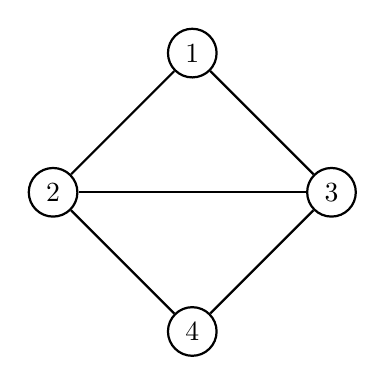
\begin{tikzpicture}[node distance={25mm}, thick, main/.style={draw,circle}]
		\node[main] (1) {$1$};
		\node[main] (2) [below left of = 1] {$2$};
		\node[main] (3) [below right of = 1] {3};
		\node[main] (4) [below right of = 2] {4};

		\draw (1) -- (2);
		\draw (1) -- (3);
		\draw (2) -- (3);
		\draw (2) -- (4);
		\draw (3) -- (4);
	\end{tikzpicture}

	\caption{Graph with multiple cycles}
\end{figure} 

\vfill

A set $F$ of edges is said to be a \textit{cut} in $G$ if there exists a partition $\{V_1, V_2\}$ of $V$ such that  $F=E(V_1, V_2)$. The edges in $F$ are said to \textit{cross} this partition. The sets $V_1 \text{ and } V_2$ are the \textit{sides} of the cut. A minimal non-empty cut in $G$ is a \textit{bond}.

\newpage

\begin{tabular}{c | c | c}
\begin{minipage}[t]{2in}
	$X=\{1\}$ \hspace{.25in} $E(1)$ \\

	\centering
	
	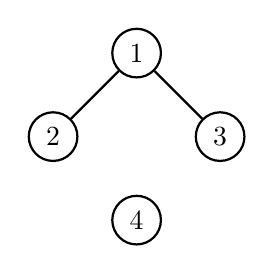
\begin{tikzpicture}[node distance={15mm}, thick, main/.style={draw,circle}]
		\node[main] (1) {$1$};
		\node[main] (2) [below left of = 1] {$2$};
		\node[main] (3) [below right of = 1] {3};
		\node[main] (4) [below right of = 2] {4};

		\draw (1) -- (2);
		\draw (1) -- (3);
	\end{tikzpicture}
\end{minipage} &
\begin{minipage}[t]{2in}
	$G[X]$ \\

	\centering
	
	
\begin{tikzpicture}[node distance={15mm}, thick, main/.style={draw,circle}]
		\node[main] (1) {$1$};
	\end{tikzpicture}
\end{minipage} &
\begin{minipage}[t]{2in}
	$G[V \setminus X]$ \\
 
	\centering
	
	\begin{tikzpicture}[node distance={15mm}, thick, main/.style={draw,circle}]
		\node[main] (2) [below left of = 1] {$2$};
		\node[main] (3) [below right of = 1] {3};
		\node[main] (4) [below right of = 2] {4};

		\draw (2) -- (4);
		\draw (2) -- (3);
		\draw (3) -- (4);
	\end{tikzpicture}
\end{minipage} \\
\end{tabular}

\vspace*{.75in}

\begin{tabular}{c | c | c}
\begin{minipage}[t]{2in}
	$X=\{2\}$ \hspace{.25in} $E(2)$ \\

	\centering
	
	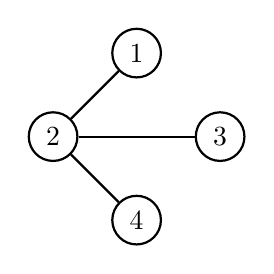
\begin{tikzpicture}[node distance={15mm}, thick, main/.style={draw,circle}]
		\node[main] (1) {$1$};
		\node[main] (2) [below left of = 1] {$2$};
		\node[main] (3) [below right of = 1] {3};
		\node[main] (4) [below right of = 2] {4};

		\draw (1) -- (2);
		\draw (2) -- (3);
		\draw (2) -- (4);
	\end{tikzpicture}
\end{minipage} &
\begin{minipage}[t]{2in}
	$G[X]$ \\

	\centering
	
	\begin{tikzpicture}[node distance={15mm}, thick, main/.style={draw,circle}]
		\node[main] (2) [below left of = 1] {$2$};
	\end{tikzpicture}
\end{minipage} &
\begin{minipage}[t]{2in}
	$G[V \setminus X]$ \\
 
	\centering
	
	\begin{tikzpicture}[node distance={15mm}, thick, main/.style={draw,circle}]
		\node[main] (1) {$1$};
		\node[main] (3) [below right of = 1] {3};
		\node[main] (4) [below right of = 2] {4};

		\draw (1) -- (3);
		\draw (1) -- (4);
	\end{tikzpicture}
\end{minipage} \\
\end{tabular}

\vspace*{.75in}

\begin{tabular}{c | c | c}
\begin{minipage}[t]{2in}
	$X=\{3\}$ \hspace{.25in} $E(3)$ \\

	\centering
	
	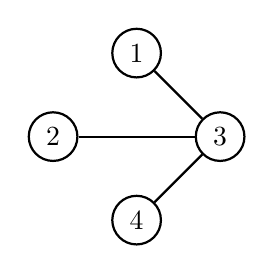
\begin{tikzpicture}[node distance={15mm}, thick, main/.style={draw,circle}]
		\node[main] (1) {$1$};
		\node[main] (2) [below left of = 1] {$2$};
		\node[main] (3) [below right of = 1] {3};
		\node[main] (4) [below right of = 2] {4};

		\draw (1) -- (3);
		\draw (2) -- (3);
		\draw (3) -- (4);
	\end{tikzpicture}
\end{minipage} &
\begin{minipage}[t]{2in}
	$G[X]$ \\

	\centering
	
	\begin{tikzpicture}[node distance={15mm}, thick, main/.style={draw,circle}]
		\node[main] (3) [below right of = 1] {3};
	\end{tikzpicture}
\end{minipage} &
\begin{minipage}[t]{2in}
	$G[V \setminus X]$ \\
 
	\centering
	
	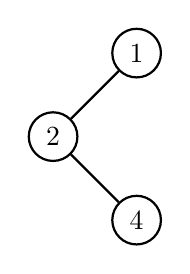
\begin{tikzpicture}[node distance={15mm}, thick, main/.style={draw,circle}]
		\node[main] (1) {$1$};
		\node[main] (2) [below left of = 1] {$2$};
		\node[main] (4) [below right of = 2] {4};

		\draw (1) -- (2);
		\draw (2) -- (4);
	\end{tikzpicture}
\end{minipage} \\
\end{tabular}

\vspace*{.75in}

\begin{tabular}{c | c | c}
\begin{minipage}[t]{2in}
	$X=\{4\}$ \hspace{.25in} $E(4)$ \\

	\centering
	
	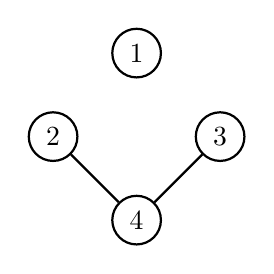
\begin{tikzpicture}[node distance={15mm}, thick, main/.style={draw,circle}]
		\node[main] (1) {$1$};
		\node[main] (2) [below left of = 1] {$2$};
		\node[main] (3) [below right of = 1] {3};
		\node[main] (4) [below right of = 2] {4};

		\draw (2) -- (4);
		\draw (3) -- (4);
	\end{tikzpicture}
\end{minipage} &
\begin{minipage}[t]{2in}
	$G[X]$ \\

	\centering
	
	\begin{tikzpicture}[node distance={15mm}, thick, main/.style={draw,circle}]
		\node[main] (4) [below right of = 2] {4};
	\end{tikzpicture}
\end{minipage} &
\begin{minipage}[t]{2in}
	$G[V \setminus X]$ \\
 
	\centering
	
	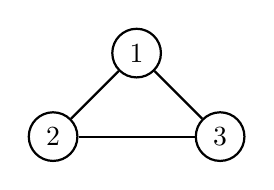
\begin{tikzpicture}[node distance={15mm}, thick, main/.style={draw,circle}]
		\node[main] (1) {$1$};
		\node[main] (2) [below left of = 1] {$2$};
		\node[main] (3) [below right of = 1] {3};

		\draw (1) -- (3);
		\draw (1) -- (2);
		\draw (2) -- (3);
	\end{tikzpicture}
\end{minipage} \\
\end{tabular}

\vfill

\begin{rem}
	A basis for the \textit{bond space} is $\{E(1), E(2), E(4)\}$.
\end{rem}

\newpage

\begin{tabular}{c | c | c}
\begin{minipage}[t]{2in}
	$X=\{1,3\}$ \hspace{.25in} $E(1) + E(3)$ \\

	\centering
	
	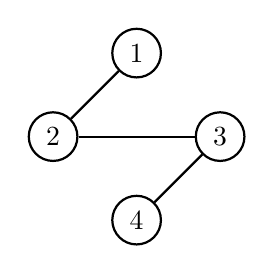
\begin{tikzpicture}[node distance={15mm}, thick, main/.style={draw,circle}]
		\node[main] (1) {$1$};
		\node[main] (2) [below left of = 1] {$2$};
		\node[main] (3) [below right of = 1] {3};
		\node[main] (4) [below right of = 2] {4};

		\draw (1) -- (2);
		\draw (2) -- (3);
		\draw (3) -- (4);
	\end{tikzpicture}
\end{minipage} &
\begin{minipage}[t]{2in}
	$G[X]$ \\

	\centering
	
	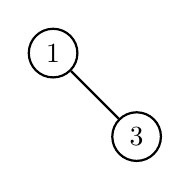
\begin{tikzpicture}[node distance={15mm}, thick, main/.style={draw,circle}]
		\node[main] (1) {$1$};
		\node[main] (3) [below right of = 1] {3};

		\draw (1) -- (3);
	\end{tikzpicture}
\end{minipage} &
\begin{minipage}[t]{2in}
	$G[V \setminus X]$ \\
 
	\centering
	
	\begin{tikzpicture}[node distance={15mm}, thick, main/.style={draw,circle}]
		\node[main] (2) [below left of = 1] {$2$};
		\node[main] (4) [below right of = 2] {4};

		\draw (2) -- (4);
	\end{tikzpicture}
\end{minipage} \\
\end{tabular}

\vspace*{.75in}

\begin{tabular}{c | c | c}
\begin{minipage}[t]{2in}
	$X=\{1,2\}$ \hspace{.25in} $E(1) + E(2)$ \\

	\centering
	
	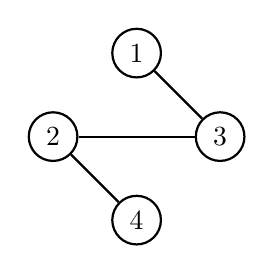
\begin{tikzpicture}[node distance={15mm}, thick, main/.style={draw,circle}]
		\node[main] (1) {$1$};
		\node[main] (2) [below left of = 1] {$2$};
		\node[main] (3) [below right of = 1] {3};
		\node[main] (4) [below right of = 2] {4};

		\draw (1) -- (3);
		\draw (2) -- (3);
		\draw (2) -- (4);
	\end{tikzpicture}
\end{minipage} &
\begin{minipage}[t]{2in}
	$G[X]$ \\

	\centering
	
	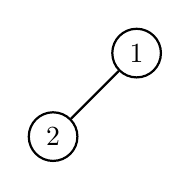
\begin{tikzpicture}[node distance={15mm}, thick, main/.style={draw,circle}]
		\node[main] (1) {$1$};
		\node[main] (2) [below left of = 1] {$2$};

		\draw (1) -- (2);
	\end{tikzpicture}
\end{minipage} &
\begin{minipage}[t]{2in}
	$G[V \setminus X]$ \\
 
	\centering
	
	\begin{tikzpicture}[node distance={15mm}, thick, main/.style={draw,circle}]
		\node[main] (3) [below right of = 1] {3};
		\node[main] (4) [below right of = 2] {4};

		\draw (3) -- (4);
	\end{tikzpicture}
\end{minipage} \\
\end{tabular}

\vspace*{.75in}

\begin{tabular}{c | c | c}
\begin{minipage}[t]{2in}
	$X=\{1,4\}$ \hspace{.25in} $E(1) + E(4)$ \\

	\centering
	
	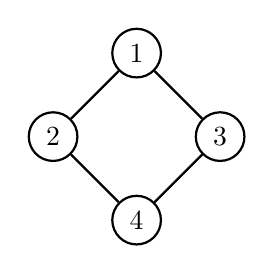
\begin{tikzpicture}[node distance={15mm}, thick, main/.style={draw,circle}]
		\node[main] (1) {$1$};
		\node[main] (2) [below left of = 1] {$2$};
		\node[main] (3) [below right of = 1] {3};
		\node[main] (4) [below right of = 2] {4};

		\draw (1) -- (2);
		\draw (2) -- (4);
		\draw (1) -- (3);
		\draw (3) -- (4);
	\end{tikzpicture}
\end{minipage} &
\begin{minipage}[t]{2in}
	$G[X]$ \\

	\centering
	
	\begin{tikzpicture}[node distance={15mm}, thick, main/.style={draw,circle}]
		\node[main] (1) {$1$};
		\node[main] (4) [below right of = 2] {4};

	\end{tikzpicture}
\end{minipage} &
\begin{minipage}[t]{2in}
	$G[V \setminus X]$ \\
 
	\centering
	
	\begin{tikzpicture}[node distance={15mm}, thick, main/.style={draw,circle}]
		\node[main] (2) [below left of = 1] {$2$};
		\node[main] (3) [below right of = 1] {3};

		\draw (2) -- (3);
	\end{tikzpicture}
\end{minipage} \\
\end{tabular}

\vfill

\begin{rem} \leavevmode
	\begin{itemize}
		\item The last cut $E(1)+E(4)$ is the only example of our graph that is not a minimal cut. Notice that this cut is the disjoint union $E(1) \dot\cup E(4)$.
		\item The induced graph $G[X]$ is disconnected and $G[V \setminus X]$ is connected.
		\item The edges that cross the cut form a cycle.
	\end{itemize}
\end{rem}

\newpage

\begin{lemma}
	Every non-minimal cut is a disjoint union of bonds.
\end{lemma}

\begin{thm}
	In a connected graph $G$, a nonempty edge cut is a bond if and only if $G[X]$ and $G[V \setminus X]$ are connected.
\end{thm}

\begin{prop}[Cut Space / Bond Space]
	Together with the $\emptyset$, the cuts in $G$ from a subspace $\mathcal{B}(G) \subseteq \mathcal{V}(E)$. This space is generted by cuts of the form $E(v)$, where $v \in V$.
\end{prop}

We define the cycle space $\mathcal{C}$ to be the subspace spanned by the edge sets of all cycles in $G$. The dimension of the cycle space is referred to as the \textit{cyclomatic number} of $G$.

\begin{prop}
TFAE for $D \subset E$:

\begin{enumerate}
	\item[(a)] D $\in \mathcal{C}(G)$
	\item[(b)] $D$ is a  possible empty disjoint union of edge sets of cycles in $G$.
	\item[(c)] All vertex degrees of the graph $(V, D)$ are even.
\end{enumerate}
\end{prop}

\newpage

\section{Minimal Spanning Trees}

\begin{defn}[Minimal Spanning Trees]
Let $G$ be a connected edge weighted graph. A minimum spanning tree (MST) of $G$ is a subset of the edges traversing all vertices, with the minimal possible total edge weight, and is acyclic.
\end{defn}

We now consider a weighted version of our graph:

\begin{figure}[h]
	\centering
	
	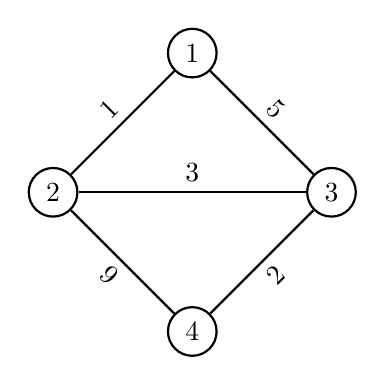
\begin{tikzpicture}[node distance={25mm}, thick, main/.style={draw,circle}]
		\node[main] (1) {$1$};
		\node[main] (2) [below left of = 1] {$2$};
		\node[main] (3) [below right of = 1] {3};
		\node[main] (4) [below right of = 2] {4};

		\draw (1) -- node[midway, above, sloped] {1} (2);
		\draw (1) -- node[midway, above, sloped] {5} (3);
		\draw (2) -- node[midway, above] {3} (3);
		\draw (2) -- node[midway, below, sloped] {9} (4);
		\draw (3) -- node[midway, below, sloped] {2} (4);
	\end{tikzpicture}

	\caption{Weighted Graph}
\end{figure} 

\begin{prop}[Cut Property]
For any cut $K$ of $G$, the edge in $K$ with the least (strictly smaller than all others) weight must belong to all MST.
\end{prop}

\begin{prop}[Cycle Property]
Given a cycle $C$ in $G$, the edge in $C$ with the largest weight cannot belong to an MST.
\end{prop}

\begin{prop}[Minimum Weight Edge Property]
If the edge with the least weight is unique, then this edge belongs to every MST.
\end{prop}


\end{document}
